%-------------------------------------------------------------------------------
% DEFINITIONS
%-------------------------------------------------------------------------------
\subsection{Définition du problème}

% LEFT-HAND SIDE
\begin{minipage}[b]{0.3\linewidth}
\centering
\includegraphics[height=3cm]{../images/salesman2.jpg}
\end{minipage}
% RIGHT-HAND SIDE
\hspace{0.5cm}
\begin{minipage}[b]{0.7\linewidth}
Le problème du Voyager de Commerce, ou \og Travelling Salesman Problem \fg{} en Anglais, consiste en l'optimisation du cout totale d'un cycle Hamiltonien\footnote{cycle Hamiltonien : passant une fois par chaque sommet.} dans un graphe complet. Nous pouvons le voir plus intuitivement comme la recherche du plus court circuit permettant de visiter un ensemble de villes.
\end{minipage}

L'équation \ref{tsp_model} montre comment le problème du Voyageur de Commerce peut se modéliser mathématiquement, où $K_n=(X,E)$ le graphe complet à $n$ sommets, $c_{ij}$ le cout de l'arête $(i,j)$ et $x_{i,j} = 1$ si notre commerçant emprunte l'arête $(i,j)$ pour faire son tour. 

\begin{equation}
\label{tsp_model}
\begin{cases}
min \sum_{\{i, j\} \in E} c_{ij}.x_{ij} \\
\sum_{i=0}^n \sum_{j=0}^n x_{ij} = 1 \\
\forall (S, \bar{S}) \sum_{i \in S, j \in \bar{S}} x_{ij} \geq 1 \\
x_{ij} \in \{0, 1\} \\
\end{cases}
\end{equation}


%-------------------------------------------------------------------------------
% SOUS-PROBLÈME
%-------------------------------------------------------------------------------
\subsection{Sous-problème}

Soit $S \subseteq X$ un sous-ensemble de sommets du graphe, avec $0 \in S$. Notons $C(S,i)$ la longueur d'une plus courte chaîne partant de $0$, arrivant au sommet $i \not\in S$ passant une et une seule fois par tout sommet de $S$ et qui n'utilise pas de sommets de $X \setminus S$ autre que $i$. 

Comme nous avons maintenant l'habitude, nous partirons de $C({0}, i)$, égale évidement à $c_{0,i}$ $\forall i$, pour essayer d'étendre le sous-problème jusqu'à arriver au problème complet~: quand nous connaissons $C(X,i)$ pour tout $i$ il suffit de choisir quelle $i$ prendre comme dernier sommet de tour, et d'ajouter alors le cout de revenir à $0$, soit $c_{i,0}$. Tout ceci est formalisé par l'équation \ref{tsp_C_optimal}, et illustré par la figure \ref{extension_tsp_chemins}.

\begin{equation}
\label{tsp_C_optimal}
C^* = min_{i \in X}[ C(X \setminus \{i\},i) + c_{i,0} ]
\end{equation}

\begin{figure}[!ht]
\begin{center}
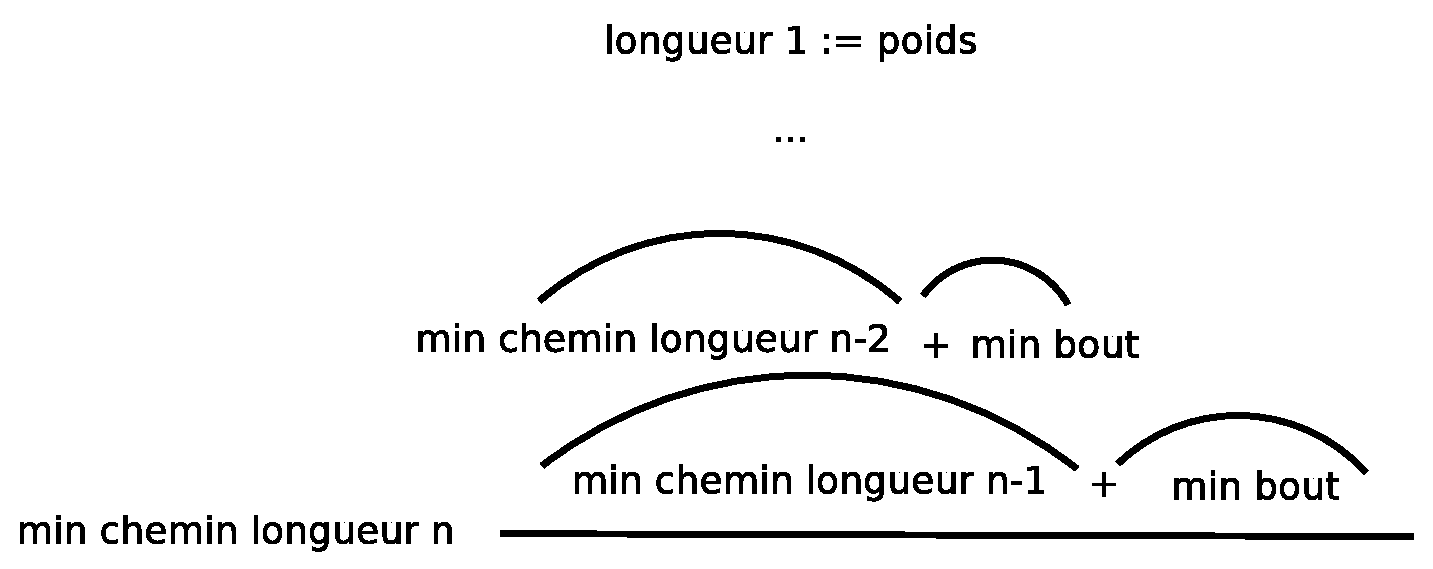
\includegraphics[height=5cm]{../images/tspDyn.eps}
\end{center}
\caption{Extension itératif des sous-TSP}
\label{extension_tsp_chemins}
\end{figure}

Pour étendre l'ensemble des sommets considérés de $S$ à $S \cup {k}$ il suffit de noter que, connaissant $C(S,i)$ pour tout $i$, nous pouvions choisir $m \in S$ tel que le cout de l'arrête $(m,k)$ plus le cout de la meilleur chaine parcourant S et s'arrêtant en $m$ soit minimale. L'équation \ref{tsp_dyn_reccurence} explicite cette relation~:

\begin{equation}
\label{tsp_dyn_reccurence}
C(S, i) =
\begin{cases}
c_{0,i} \text{ si } S = \{0\} \\
min_{m \in S, k \not\in S}[ C(S\setminus\{m\}, k) + c_{m,k} ] \text{ sinon}
\end{cases}
\end{equation}

%-------------------------------------------------------------------------------
% ALOGORITHM
%-------------------------------------------------------------------------------
\subsection{Algorithme}

Nous proposons l'algorithme suivant pour une programmation dynamique
du TSP.

\begin{algorithm}[!ht]
\caption{Programmation dynamique pour le TSP}
\label{Dyntsp}
\begin{algorithmic}[1]
\REQUIRE une matrice de poids, un ensemble de $n$ sommets
\FOR{chaque sous-ensemble $S$ commençant par $0$}
\IF{$|S| = 2$}
\FOR{$i$ de $0$ à $n-1$}
\STATE C[S][i] := poids[0][i]
\ENDFOR
\ELSE
\FOR{$i$ de $0$ à $n-1$}
\FOR{tous les $k$ $\notin$ $S - \{ 0 \}$}
\STATE C[S][i] := $\min$ $\{$ C[$S - \{ k \} $][k] + poids[k][i] $\}$
\ENDFOR
\ENDFOR
\ENDIF
\ENDFOR
\STATE retourner $\min$ $\{$ C[S][i] + poids[i][0] $\}$ avec $|S| = $
(nombre de sommets - 1)
\end{algorithmic}
\end{algorithm}

La complexité théorique d'un tel algorithme est de $O(n^2.2^n)$.

%-------------------------------------------------------------------------------
% IMPLEMENTATION
%-------------------------------------------------------------------------------
\subsection{Implémentation en \texttt{C++}}

Nous avions choisi le \texttt{C++} à fin de bénéficier des structures \texttt{std::map}, texttt{std::pair} et surtout \texttt{std::set} de la STL\footnote{STL : standard \texttt{C++} library.}. Ces structures sont bien implémentés avec accès logarithmique. Cependant pour utiliser des ensembles comme clefs d'ensembles\footnote{les arbres de recherche sont utilisés, avec une opération de comparaison appliqué récursivement sur les meta-ensembles.} il faut faire un nombre important de copies locales, donc des opérations linéaires. 

Cette implémentation ne respecte donc certainement pas le facteur quadratique, mais l'important, l'exponentielle, est respecté~:

\vspace{0.5cm}

\lstinputlisting[language=C++,morekeywords={}]{../code/salesman.cpp} 

%-------------------------------------------------------------------------------
% TESTS
%-------------------------------------------------------------------------------
\subsection{Tests et conclusion}
Nous mesurons ici une moyenne du temps d'exécution sur 5 tests en faisant varier le nombre de sommets à parcourir. Le faible nombre de tests provient simplement du fait que l'exécution d'un seul peut prendre plusieurs minutes même qu'avec une dizaine de sommets. Les résultats obtenues sont présentés dans les figures \ref{tsp_graph} et \ref{tsp_table}

\begin{figure}[ht]
% LEFT-HAND SIDE
\begin{minipage}[b]{0.5\linewidth}
\centering
\begin{tikzpicture}[scale=0.9]
    \begin{axis}[title=Jeux de tests pour le TSP, xlabel= nombre de
        villes parcourues, ylabel= temps d'exécution]
      \addplot
        table[col sep=comma]{../charts/tspdyn.csv};
        %\legend{exécution du tsp}
    \end{axis}
\end{tikzpicture}
\caption {Courbe des temps d'exécution pour TSP}
\label{tsp_graph}
\end{minipage}
% RIGHT-HAND SIDE
\hspace{0.5cm}
\begin{minipage}[b]{0.5\linewidth}
\centering
\begin{tabular}{|c|c|}
\hline
Sommets & t moyenne en ms\\
\hline
2 & $\simeq 0$\\
\hline
5 & 2\\
\hline
7 & 15\\
\hline
9 & 137\\
\hline
11 & 1151\\
\hline
13 & 8575\\
\hline
15 & 58109\\
\hline
\end{tabular}
\caption {Tableau des temps d'exécution pour TSP}
\label{tsp_table}
\end{minipage}
\end{figure}

Nous voyons que cette algorithme exponentielle n'est pas opérationnelle pour des instances de taille au dessus d'une vingtaine. Pour 60 sommets, par exemple, il sera question de l'ordre de 130 millénaires de calculs avec une opération par nanoseconde. 

Pour ces grands instances nous n'avions donc d'autre choix que les méthodes approchés, enfin presque\dots

\begin{figure}[h!]
\centering
\includegraphics[width=0.9\textwidth]{../images/salesman1.png}
\end{figure}